
% VYSOKOŠKOLSKÁ KVALIFIKAČNÍ PRÁCE
% autor: Michal Struna
% název: Webový 3D simulátor těles ve vesmíru
% kódování zdroje: UTF-8

\documentclass[a4paper,12pt]{article}

\usepackage{vskpupa}	% globální nastavení pro text VŠKP UPa
\usepackage{listings}
\def\code#1{\texttt{#1}}
\setlist{itemsep=0pt,topsep=2pt} % TODO: Refactor.
\renewcommand{\lstlistingname}{Zdrojový kód}
\renewcommand{\lstlistlistingname}{Seznam zdrojových kódů}

\usepackage{color}
\definecolor{lightgray}{rgb}{.9,.9,.9}
\definecolor{darkgray}{rgb}{.4,.4,.4}
\definecolor{gray}{rgb}{0.6, 0.6, 0.6}

\titleformat{\section}
	{\Large\bfseries}
	{\thesection}
	{1em}
	{\MakeUppercase}		% titulky sekcí verzálkami
\titleformat*{\subsection}{\large\rmfamily\bfseries}
\titleformat*{\subsubsection}{\normalsize\rmfamily\bfseries}

\usepackage{float}

\lstdefinelanguage{JavaScript}{
  keywords={this, const, let, class, extends, export, default, public, static, typeof, new, true, false, catch, function, return, null, catch, switch, var, if, in, while, do, else, case, break},
  keywordstyle=\color{blue}\bfseries,
  identifierstyle=\color{black},
  sensitive=false,
  comment=[l]{//},
  morecomment=[s]{/*}{*/},
  commentstyle=\color{gray}\ttfamily,
  stringstyle=\color{red}\ttfamily,
  morestring=[b]',
  morestring=[b]"
}

\lstset{
   language=JavaScript,
   extendedchars=true,
   basicstyle=\footnotesize\ttfamily,
   showstringspaces=false,
   showspaces=false,
   tabsize=2,
   breaklines=true,
   showtabs=false,
   captionpos=b
}

% ÚDAJE O PRÁCI
\def\jmenoFakulty{Fakulta elektrotechniky a informatiky}
\def\jmenoAutora{Michal Struna}
\def\nazevPrace{Webový 3D simulátor těles ve vesmíru}
\def\typPrace{Bakalářská práce}
\def\rok{2019}
% cesty k obrázkům zadání, je-li zadání naskenováno
\def\prefixZadani{Images/zadani}	% cesta a začátek jména, bude doplněno číslo strany
\def\suffixZadani{.jpg}		% doplní se ke každému jménu souboru zadání
\def\datumOdevzdaniPrace{?.\,?.\,2019}

\usepackage{lipsum}		% \lipsum[číslo] vloží jeden odstavec Lorem ipsum…
% \usepackage[none]{hyphenat}

\long\def\textPodekovani{%
	\lipsum[1]		% nahradit makro \lipsum skutečným textem
}

\long\def\anotace{
	Bakalářská práce se v~praktické části zabývá implementací webové aplikace pro 3D~vizualizaci těles ve vesmíru. V~rámci aplikace je kladen důraz na dynamický obsah, na kterém se mohou všichni uživatelé po úspěšně autentifikaci podílet. Veškerý obsah je možné pomocí serverového REST API upravovat. Teoretická část je zaměřena na popis technologií pro tvorbu webových aplikací, vysvětlení životního cyklu aplikace a~uvedení řešení několika problémů spojených s~implementací. Součástí teoretické části je také detailní popis všech stránek nacházejících se v aplikaci.
}
\def\klicovaSlova{webová aplikace, simulátor, vesmír, astronomie, TypeScript, 3D}
\def\title{Web 3D simulator of bodies in universe}
\long\def\annotation{
	The bachelor thesis in practical parts deals with implementation of web applications for 3D~visualization of bodies in space. Within the application, emphasis is placed on the dynamic content on which all users can participate after successful authentication. All content can be edited using the REST~API. The~theoretical part focuses on the description of technologies for creating web applications, explaining the life cycle of the~application and introducing solutions to several problems connected with implementation. Part of the theoretical part is also a~detailed description of all the pages that are in the~application.
}
\def\keywords{web application, simulator, universe, astronomy, TypeScript, 3D}


% VYZNAČOVÁNÍ
% odkomentovat v případě potřeby
%\usepackage{ulem}\normalem		% potrhávání, \emph se bude chovat normálně (kurziva)
%\usepackage[letterspace=400]{microtype}	% prostrkávání
%\definecolor{red}{cmyk}{0, 1, 1, 0.3}	% redefinice červené barvy (použito pro pro vyznačování)

%\let\uv\autouv				% odkomentovat pro automatické vnořené jednoduché uvozovky

%%%%%%%%%%%%%%%%%%%%%%%%%%%%%%%%%%%%%%%%%%%%%%%%%%%%%%%%%%%%
% NASTAVENÍ HYPERTEXTOVÝCH ODKAZŮ
%%%%%%%%%%%%%%%%%%%%%%%%%%%%%%%%%%%%%%%%%%%%%%%%%%%%%%%%%%%%

% a) výchozí nastavení: rámečky kolem textu, které se netisknou

% b) bez rámečků, odkomentovat:
%\hypersetup{hidelinks}

% c) bez rámečků, barevně, odkomentovat:
%\hypersetup{
%	colorlinks=true,	% zapnout barvy, vypnout rámečky
%	% nastavit barvy samostatně:
%	linkcolor=red,		% interní odkazy (křížové reference)
%	anchorcolor=black,	% text kotvy
%	citecolor=green,	% text odkazu na citaci
%	filecolor=cyan,		% URL pro lokální soubory
%	urlcolor=magenta,	% URL
%	% nebo nastavit všechny barvy stejně:
%	%allcolors=blue, 	% všechny odkazy (netýká se rámečků)
%}

% další vlastní nastavení uživatele

%%%%%%%%%%%%%%%%%%%%%%%%%%%%%%%%%%%%%%%%%%%%%%%%%%%%%%%%%%%%
% ZAČÁTEK DOKUMENTU
%%%%%%%%%%%%%%%%%%%%%%%%%%%%%%%%%%%%%%%%%%%%%%%%%%%%%%%%%%%%

\begin{document}

%%%%%%%%%%%%%%%%%%%%%%%%%%%%%%%%%%%%%%%%%%%%%%%%%%%%%%%%%%%%
% ÚVODNÍ STRANY
%%%%%%%%%%%%%%%%%%%%%%%%%%%%%%%%%%%%%%%%%%%%%%%%%%%%%%%%%%%%

\titulniStrana			% titul

% ZADÁNÍ
%\generujZadani[2]	% parametr je počet stran, výchozí (neuvede-li se) je 2
\generujProhlaseni		% prohlášení
\generujPodekovani		% poděkování
\generujAnotaci			% anotace
\generujAnnotation		% anotace anglicky
\generujObsah			% obsah
\generujSeznamObrazku		% seznam obrázků

%%%%%%%%%%%%%%%%%%%%%%%%%%%%%%%%%%%%%%%%%%%%%%%%%%%%%%%%%%%%
% SEZNAM ZKRATEK

\clearpage \phantomsection \addcontentsline{toc}{section}{Seznam zdrojových kódů}
\lstlistoflistings

\seznamZkratek			% titulek a řádek do obsahu

% netučně, odsazení 6em (možno změnit), šířka pro pojem/zkratku se dopočítá z odsazení
\begin{description}[font=\mdseries,leftmargin=6em,labelwidth=!,]
\item[3D]		Three Dimensional
\item[API]		Application Programming Interface
\item[BSON]	Binary JSON
\item[CSS]	Cascading Style Sheets
\item[CRUD]	Create, Read, Update, Delete
\item[DOM]	Document Object Model
\item[HTML] Hypertext Markup Language
\item[HTTP]	Hypertext Transfer Protocol
\item[HW] 	Hardware
\item[JPEG]		 Joint Photographic Experts Group
\item[JS]		JavaScript
\item[JSON]	JavaScript Object Notation
\item[PNG]		Portable Network Graphics
\item[REST]	Representational State Transfer
\item[SASS]	Syntactically awesome style sheets
\item[TS]		TypeScript
\item[UI]		User Interface
\item[URI]		Uniform Resource Identifier 
\item[XML]	Extensible Markup Language
\end{description}


%%%%%%%%%%%%%%%%%%%%%%%%%%%%%%%%%%%%%%%%%%%%%%%%%%%%%%%%%%%%
% ÚVOD
%%%%%%%%%%%%%%%%%%%%%%%%%%%%%%%%%%%%%%%%%%%%%%%%%%%%%%%%%%%%

\clearpage
\pagestyle{plain}		% zapne číslování stránek (sazba zápatí)

\phantomsection \addcontentsline{toc}{section}{Úvod}
\section*{Úvod}
\label{uvod}

V~dnešní době zažívá odvětví astronomie velký rozmach. Lze nalézt mnoho portálů, které nově objevené informace ihned zveřejňují. Často se však jedná o~rozsáhlé monografie, které laikovi příliš neřeknou. Navíc ne vždy jsou dostupné v~české lokalizaci. Na druhé straně existují 3D~simulátory, které je ale nutno stahovat z~internetu a~poté instalovat. Tyto simulátory však obsahují pouze minimum informací a~spíše než informační prostředek a~komunitní portál slouží jako pouhá vizuální scéna.

Cílem této bakalářské práce, je vytvořit aplikaci, která poskytne jednoduchý pohled na astronomii lidem, kteří by se o~tomto odvětví něco rádi  dozvěděli. Díky obsáhlé databázi dat však nabízí i~pohodlný a~dostupný zdroj informací pro pokročiĺejší uživatele. Spojuje tak textové zdroje a~grafické aplikace. Uživatel má možnost 
si libovolnou vlastnost libovolného tělesa zobrazit graficky před sebou a~tuto vlastnost pak porovnat napříč všemi tělesy v~databázi. Vše je dostupné v~české lokalizaci a~zároveň je celá aplikace online.

Obsah webové aplikace je plně dynamický a~kdokoliv do něj může přispívat svými znalostmi. Všechny takto přidané informace však prochází schvalovacím procesem, kterého se účastní administrátor.


%%%%%%%%%%%%%%%%%%%%%%%%%%%%%%%%%%%%%%%%%%%%%%%%%%%%%%%%%%%%
% KAPITOLY
%%%%%%%%%%%%%%%%%%%%%%%%%%%%%%%%%%%%%%%%%%%%%%%%%%%%%%%%%%%%

\section{3D simulace a jejich řešení}



\subsection{Celestia}

\textit{Celestia} je \textit{open-source} 3D program zobrazující tělesa ve vesmíru v reálném čase. Podobně jako tato bakalářská práce obsahuje databázi těles od těch nejmenších meteoritů až po celé galaxie. Vzhledem k tomu, že program Celestia vyvíjí komunita a~nikoliv jednotlivec je tato databáze mnohem rozsáhlejší a~lze si dodatečně stáhnout více jak 10 GB dat.

Program je vytvořen v~\textit{C++} a \textit{Lua}, což mu dovoluje výkon počítače využívat podstatně lépe, než webová aplikace. Navzdory tomu je nutno tento program nejdříve nainstalovat, což může některé uživatele odradit. Je však dostupný jak pro \textit{Windows}, tak i~pro \textit{Linux} a~\textit{macOS}. Neobsahuje ovšem češtinu. 

\begin{figure}[H]
  \centering
  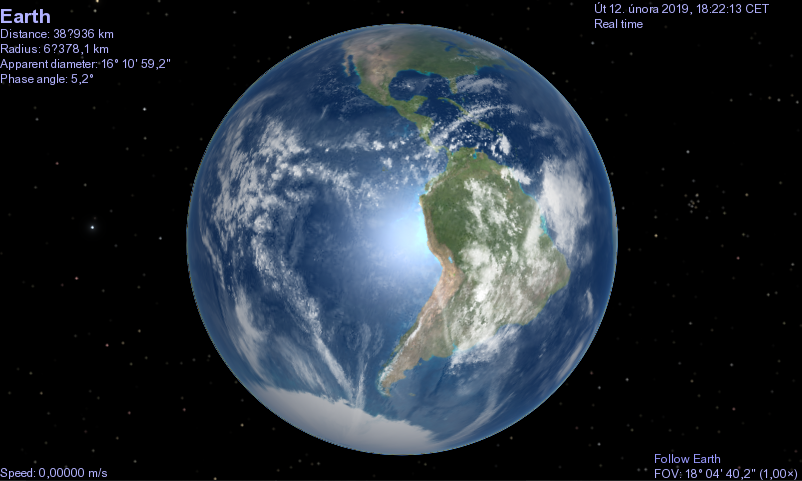
\includegraphics[width=450pt]{Images/Celestia.png}
  \caption[Ukázka programu Celestia]{Ukázka JPL Solar Simulator  \footnotemark[1]}
\end{figure}

\footnotetext[1]{Fotografie pořízena z programu Celestia (\url{https://celestia.space/}).}

\subsection{Stellarium}

\textit{Stellarium} je dalším z řady \textit{open-source} astronomických programů. Není zde však možné se volně pohybovat prostorem. Program se specializuje na zobrazování oblohy, a~to v~jakoukoliv dobu jakéhokoliv dne z~jakéhokoliv místa na Zemi.

Obsahuje velice rozsáhlou databázi obsahující v~základní instalaci necelý milion těles. Je však možné si dodatečně nainstalovat katalogy s~více jak 200 miliony tělesy. U každého tělesa je možné si zobrazit stručné informace, především co se jejich polohy a~vzdálenosti od Země týče.

Jedná se o~program napsaný v~\textit{C++}, což stejně jako u~programu Celestia vede k~vysokému výkonu, avšak nutnosti instalace. Je ovšem dostupný i~v~české lokalizaci a opět pro \textit{Windows}, \textit{Linux} i~\textit{macOS}.

\begin{figure}[H]
  \centering
  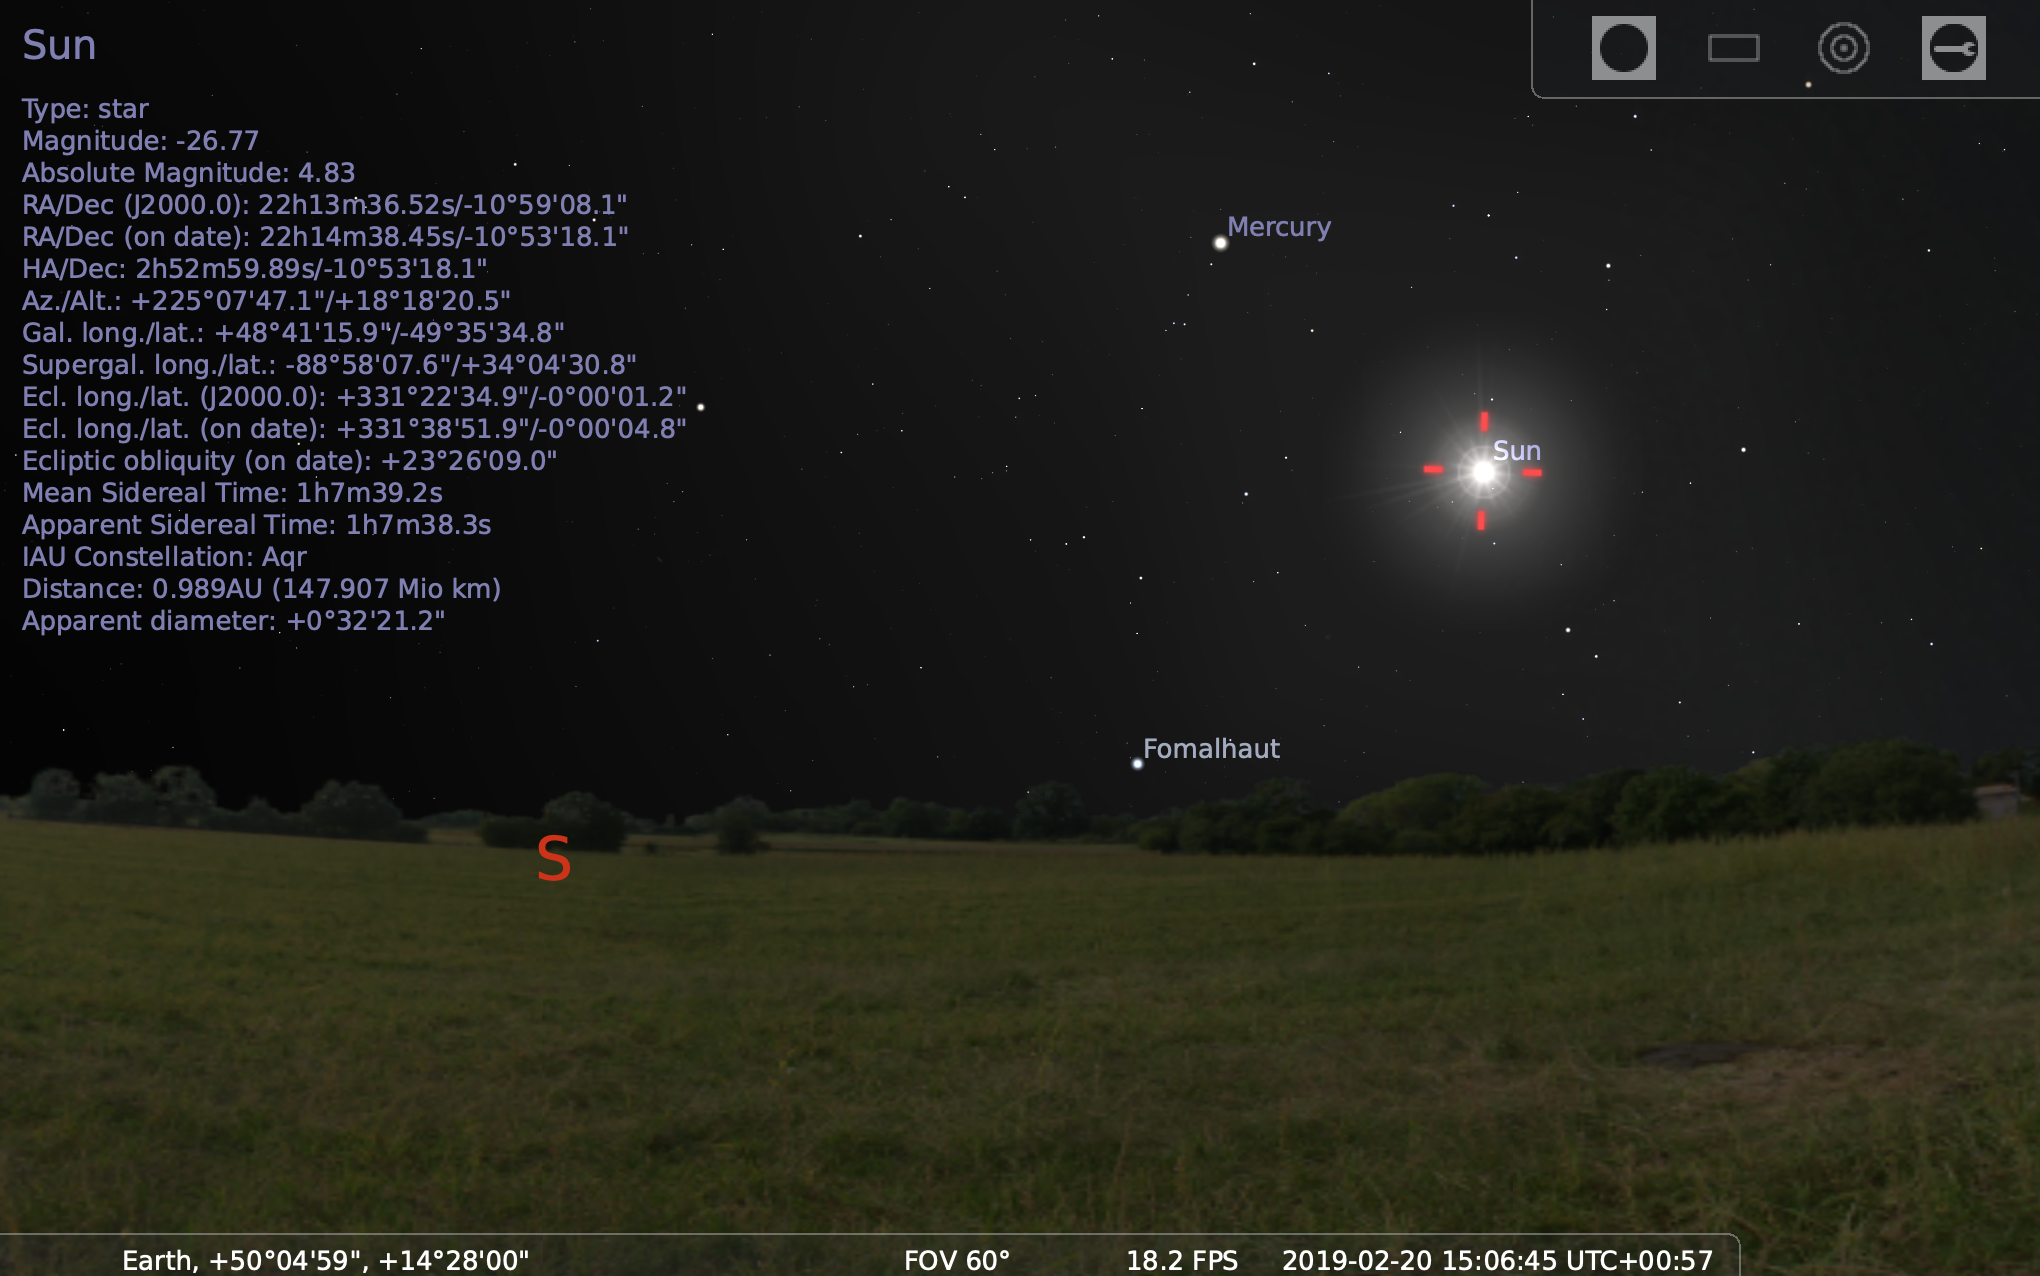
\includegraphics[width=450pt]{Images/Stellarium.png}
  \caption[Ukázka programu Stellarium]{Ukázka programu Stellarium  \footnotemark[1]}
\end{figure}

\subsection{NASA/JPL Solar System Simulator}

Jedná se o~webovou aplikaci, která umožňuje zobrazit libovolné těleso v~databázi libovolnou dobu a~to z~libovolného jiného tělesa v~databázi. Obsahuje pouze tělesa z~naší sluneční soustavy. Umožňuje nastavit i~velikost zorného pole ve stupních. Vygenerovaný pohled je ale bohužel pouze statický a~nelze s~ním už dál nijak interagovat.

\begin{figure}[H]
  \centering
  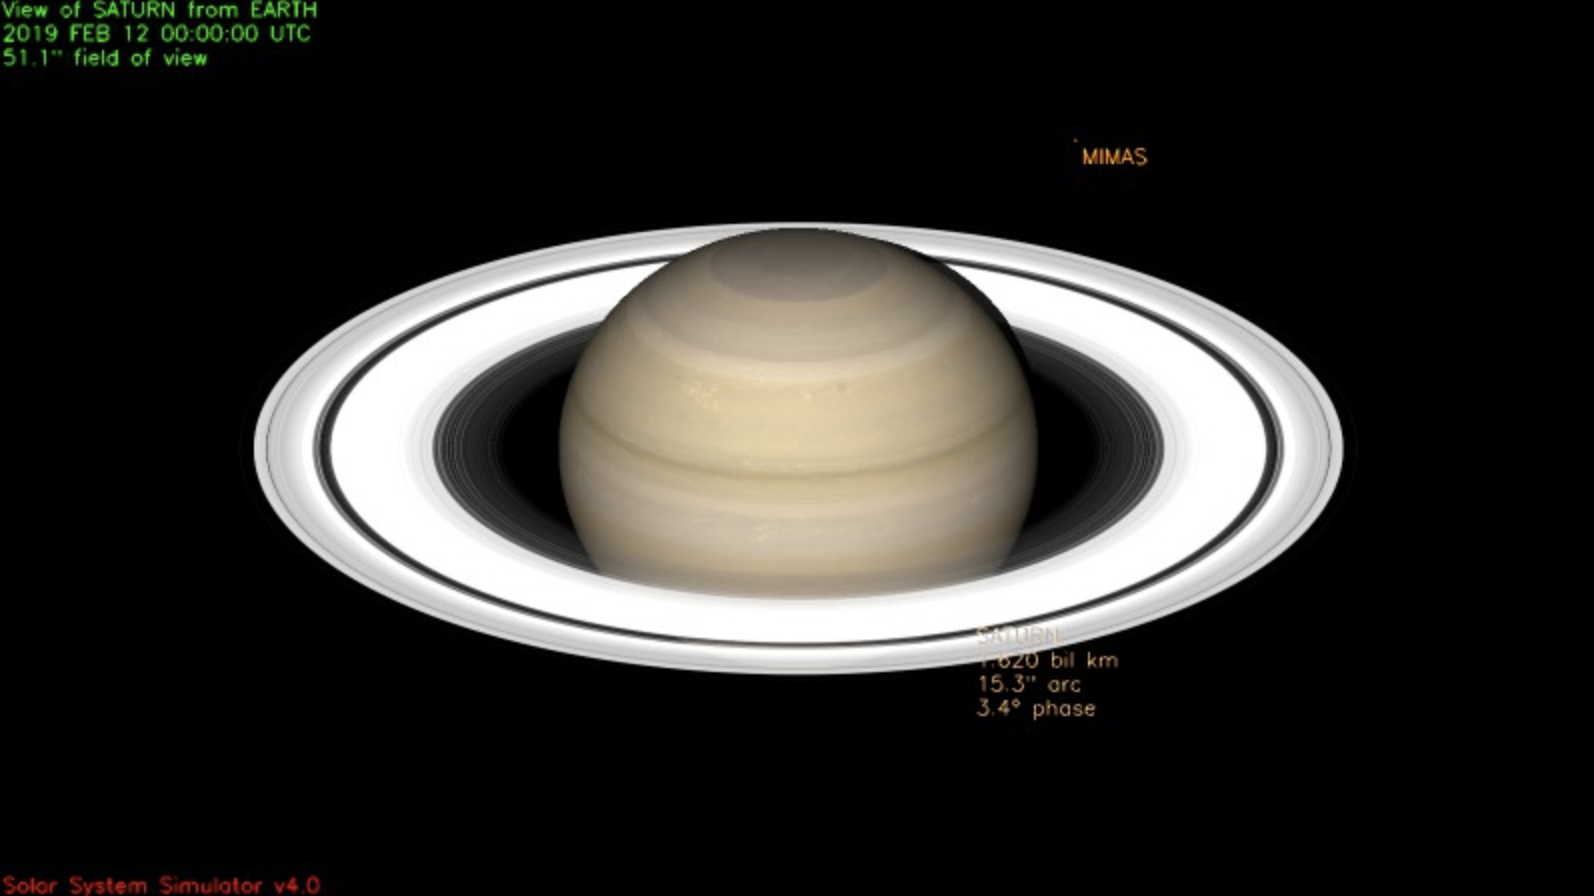
\includegraphics[width=450pt]{Images/JPLNasa.png}
  \caption[Ukázka JPL Solar System Simulator]{Ukázka JPL Solar Simulator   \footnotemark[2]}
\end{figure}

\footnotetext[1]{Fotografie pořízena z programu Stellarium (\url{https://stellarium.org}).}
\footnotetext[2]{Fotografie pořízena z \url{https://space.jpl.nasa.gov/}.}

\subsection{Space Engine}
\subsection{Universe Sandbox}


\section{Použité technologie}

\subsection{Jazyk TypeScript}

\textit{TypeScript} je programovací jazyk vyvinutý firmou \textit{Microsoft}. Jedná se o~nádstavbu jazyka \textit{JavaScript}, která přidává statické typování a~další vlastnosti objektového programování. Kód napsaný v~jazyce \textit{JavaScript} je kompatibilní s~\textit{typescriptovým} kódem. Pro kompatibilitu v~prohlížečích je nutné veškerý \textit{TypeScript} transpilovat do \textit{javascriptového} kódu.~\cite{typescript}

\subsection{Knihovna React}

Javascriptová knihovna \textit{React}, jejíž autorem je \textit{Facebook}, usnadňuje a~zefektivňuje tvorbu \textit{UI}.~\cite{react} Přináší tzv. \textit{one-way data binding}, které zaručuje okamžitou aktualizaci \textit{UI} při změně stavu aplikace.~\cite{onewaydatabinding} \textit{React} si vytváří vlastní virtuální \textit{DOM}, který je na rozdíl od toho v~\textit{HTML} rychlejší. V tomto modelu pak React provádí všechny své operace. Teprve když je třeba provést změnu v~prohlížeči, je třeba  aktualizovat \textit{HTML}.~\cite{virtualdom}

\subsubsection{Syntaxe JSX}

Vytvářet zanořovací strukturu komponent může být nepřehledné. Proto se často s~knihovnou \textit{React} používá i~syntaxe \textit{JSX}. Ta umožňuje psát \textit{javascriptový} kód v~podobě \textit{XML} tagů. \textit{JSX} syntaxi je z~důvodů kompatibility prohlížečů nutné transpilovat do nativního \textit{JavaScriptu}.~\cite{jsxsyntax}

\lstinputlisting[caption={Porovnání vykreslení komponenty ve standardním JavaScriptu a~v~JSX}, language={JavaScript}]{SourceCodes/JSX.js}

\subsection{Knihovna Three.js}

\textit{Three.js} je javascriptová knihovna usnadňující práci s~\textit{WebGL}. To je rozhraní, které umožňuje přístup k \textit{HW} komponentám počítače specializovaných pro zpracování grafiky 2D a~3D grafiky přes \textit{JavaScript}. Veškerou tuto grafiku je možno vykreslovat v~prohlížeči za využití elementu \code{canvas}.~\cite{three}

\subsection{Framework Node.js}

Framework \textit{Node.js} umožňuje používání jazyka \textit{JavaScript} na serveru. Pracuje pouze s~jediným vláknem a~funguje na asynchronním neblokujícím zpracování požadavků. Jakmile je dokončen požadavek, jeho callback uvedený v argumentu se zařadí do fronty.  Tzv. \textit{event loop} pak zjišťuje, zda je zásobník zpracovávaných operací prázdný. Pokud ano, vloží do něj první callback z~fronty. Tento cyklus se opakuje po celou dobu běhu serveru.~\cite{node}

\subsection{Databáze MongoDB}

\textit{MongoDB} je \textit{NoSQL} multiplatformní dokumentová databáze s~otevřeným zdrojovým kódem. Narozdíl od relačních databází používá dokumenty ve formátu \textit{BSON}, který je podobný \textit{JSON}. Při vytváření dokumentů si databáze automaticky vytváří vlastní unikátní ID.  Uložené dokumenty lze vedle porovnávání hodnot vyhledávat na základě prvků v~poli, podle rozsahu nebo podle regulárních výrazů. V~\textit{MongoDB} je možné indexovat libovolné pole dokumentů. Indexy jsou koncepčně stejné, jako v~relačních databázích.~\cite{mongomongoose}

\subsection{Knihovna Mongoose}
Open-source knihovna \textit{Mongoose} zjednodušuje práci s~MongoDB, zejména pak vytváření schémat a~validaci dat.~\cite{mongomongoose}

\subsection{Framework Swagger}
\textit{Swagger} je nástroj pro vyzualizaci \textit{REST API} z~\textit{Open API} specifikace.

\subsection{Nástroj Webpack}
Prohlížečový \textit{JavaScript} nativně nepodporuje rozdělování kódu do modulů (jako např. \textit{Java} do balíčků nebo \textit{C++} do jmenných prostorů). Jediným způsobem je importovat do \textit{HTML} větší množství \textit{javascriptových} souborů pomocí tagu \code{<script>}. Tento postup je ale špatnou praktikou a~na web má negativní dopady.~\cite{jsconcat}

Díky nástroji \textit{Webpack} je možné v~\textit{JavaScriptu} využívat modulární systémy jako \textit{CommonJS}, \textit{AMD} nebo \textit{ES modules}. Je tak možné větší množství souborů propojit pomocí klauzulí \code{require} nebo \code{import}.~\cite{webpack}

\textit{Webpack} také umožňuje využívat tzv. \textit{loadery} třetích stran. To vede k možnosti podobně načítat, slučovat či parsovat i soubory jiných typů, např. \textit{CSS}, \textit{SVG} nebo \textit{JSON}. Zároveň za využití bohaté nabídky pluginů lze všechny tyto soubory modifikovat, např. převádět nový \textit{JavaScript} verze \textit{ES6} na starší, podporovaný prohlížeči.~\cite{webpack}

\lstinputlisting[caption={Konfigurace nástroje Webpack v souboru webpack.config.json}, language={JavaScript}]{SourceCodes/Webpack.js}.

\subsection{Verzovací systém Git}

\textit{Git} je systém správy verzí vytvořený \textit{Linusem Torvaldsem}. Při vytváření nové verze dat vytvoří snímky všech souborů tak, jak v daný okamžik vypadají a~na tyto snímky pak uloží reference. V~případě, že se soubor nijak nemění se nevytváří nový snímek, ale pouze se nastaví reference na ten předchozí, který je identitický.~\cite{git}

Pro spravované soubory používá tři stavy. Při změně souboru se nastaví jeho stav na \textit{modified}. Stav \textit{staged} znamená, že soubor byl označen k tomu, aby byl zapsán v další verzi. Zapsaný soubor je ve stavu \textit{commited}. Všechny tyto změny jsou však pouze lokální. Pro umístění změn do vzdáleného repozitáře je třeba všechny zapsané soubory odeslat \textit{(push)}. Ostatní s~přístupem do repozitáře si pak mohou tyto změny stáhnout \textit{(pull)}.~\cite{git}

\subsection{Balíčkovací systém NPM}

\textit{NPM} je správce balíčků pro serverový i~klientský \textit{JavaScript}. Řídícím souborem v projektu je \textit{package.json}, který obsahuje informace o~projektu a~určuje, které balíčky jsou součástí projektu.  Všechny balíčky jsou umístěny do adresáře \textit{node\_modules} v~projektu. Součástí je také soubor \textit{package-lock.json}, který zachovává verze nainstalovaných balíčků.~\cite{npm}

\lstinputlisting[caption={Ukázka práce s~NPM}, language={JavaScript}]{SourceCodes/Npm.txt}.

\subsection{Preprocesor SASS}

Preprocesor \textit{SASS} přidává do \textit{CSS} možnost zanořování selektorů, proměnné, funkce, podmínky a~další vlastnosti zlepšující čitelnost kódu. Pro kompatibilitu s~prohlížeči je nutné ho transpilovat do \textit{CSS}.

\section{Návrh a~vývoj aplikace}

\subsection{Struktura projektu}

React nepřichází s~žádnou doporučenou strukturou projektu. Proto došlo k~vytvoření vlastní struktury. Vzhledem k~velkému množství souborů je celý obsah projektu členěn do podadresářů a~modulů.

\begin{itemize}
\item \textbf{dist}: Produkční sestavení aplikace. Veškerý obsah adresáře se generuje automaticky.
\item \textbf{node\_modules}: Externí knihovny pro serverovou část.
\item \textbf{src}: Zdrojové soubory aplikace.

\begin{itemize}
\item \textbf{Client}: Podprojekt, který obsahuje všechny klientské soubory.

\begin{itemize}
\item \textbf{node\_modules}: Externí knihovny pro klientskou část.
\item \textbf{src}:  Zdrojové soubory klientské části.

\begin{itemize}
\item \textbf{Controls}: Modul obsahující ovladače a~tlačítka využitá v~menu.
\item \textbf{Forms}: Modul umožňující tvorbu formulářů.
\item \textbf{Global}: Hlavičkové soubory dostupné v~globálním prostoru.
\item \textbf{Panel}: Modul pro panel tělesa.
\item \textbf{System}: Hlavní modul obsahující systémové soubory.
\item \textbf{Universe}: Modul zprostředkovávající simulátor.
\item \textbf{User}: Modul s~formuláři a~další komponentami pro uživatele.
\item \textbf{Utils}: Pomocný modul.
\end{itemize} 

\end{itemize} 

\item \textbf{Constants}: Konstanty a~konfigurace.
\item \textbf{Controllers}: Kontrolery s~adresářovou strukturou popisující REST~API.
\item \textbf{Database}: Databázové soubory.

\begin{itemize}
\item \textbf{Plugins}: Databázové pluginy.
\item \textbf{Schemas}: Databázová schémata.
\end{itemize} 

\item \textbf{Global}: Hlavičkové soubory dostupné v~globálním prostoru.
\item \textbf{Models}: Modelové třídy obsahující aplikační logiku.
\item \textbf{Public}: Vstupní HTML soubor a~další statické soubory.

\begin{itemize}
\item \textbf{Fonts}: Písma.
\item \textbf{Images}: Obrázky rozčleněné do podadresářů.
\item \textbf{JavaScript}: Javascriptové soubory.
\end{itemize} 

\item \textbf{Utils}:  Pomocné třídy.
\end{itemize} 

\item \textbf{docs}:  Teoretická část bakalářské práce včetně zdrojových souborů pro LaTeX.

\end{itemize} 

Moduly obsažené zejména v~klientské části projektu jsou adresářové celky, které mohou obsahovat další strukturu:

\begin{itemize}
\item \textbf{Components}: React komponenty.
\item \textbf{Constants}: Konstanty a konfigurace modulu.
\item \textbf{Redux}: Akce a reducer.
\item \textbf{Styles}: Styly.
\item \textbf{Views}: Pohledy.
\end{itemize} 

Každý modul obsahuje mapování a~export všech souborů, které mají být veřejné. Z~vnějšku tedy není nutné znát strukturu daného modulu a~adresu hledaného souboru uvnitř modulu.


\lstinputlisting[caption={Správné a~nesprávné použití importu souboru z~modulu}, language={JavaScript}]{SourceCodes/ImportFromModule.js}


\subsection{Uživatelské rozhraní}

Klientská část aplikace dodržuje architekturu \textit{Redux}. Všechen stav aplikace je na jednom místě v~tzv. \textit{store}, odkud ho mohou číst všechny komponenty, jež jsou na \textit{store} napojené. Kdykoliv se změní stav aplikace, dojde k~automatickému překreslení těch částí \textit{UI}, které změněná data obsahují.

Stav aplikace lze změnit zavoláním funkce \textit{dispatch}, jejímž argumentem bude právě prováděná akce. Akce je prostým objektem, který obsahuje povinnou vlastnost \code{type} s~typem akce a~libovolné další vlastnosti. Jelikož akce by měly být znovupoužitelné, jsou často umístěny v~\textit{action creator}. To je funkce, která akci vrací.

\begin{figure}[H]
\begin{center}
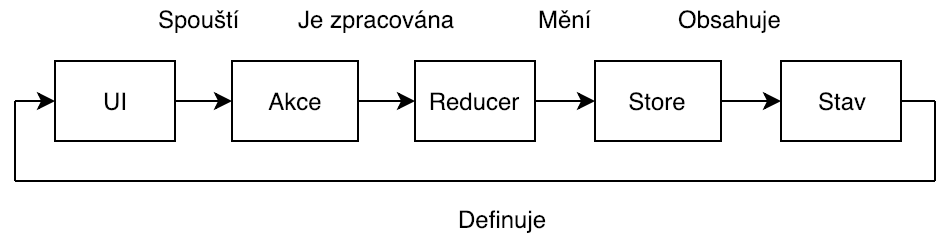
\includegraphics[width=350pt]{Images/Redux.png}
\caption[Životní cyklus architektury Redux]{Životní cyklus architektury Redux \footnotemark}
\label{BodiesList}
\end{center}
\end{figure}

\footnotetext[1]{Vytvořeno v \url{https://www.draw.io}.}

Samotná změna stavu je pak provedena ve funkci \textit{reducer}. Ten ze starého stavu aplikace a~akce vytvoří a~vrátí nový stav. Je složen obvykle z~přepínače s~výčtem všech akcí, kde je u~každé akce uvedena její modifikace stavu. Aby změna stavu aktualizovala všechny komponenty, které tomuto stavu naslouchají, je nutné, aby \textit{reducer} vracel vždy nově vytvořený objekt, nikoliv pouze pozměněný ten starý.

\lstinputlisting[caption={Ukázka architektury Redux}, language={JavaScript}]{SourceCodes/Redux.js}

\subsubsection{Akce}

Vytvářet zejména asynchronní akce manuálně je zdlouhavé. Pro správnou funkcionalitu \textit{UI} je totiž při asynchronním požadavku třeba zaznamenat následující stavy:

\begin{itemize}
\item \textbf{SENT}: Požadavek byl odeslán,
\item \textbf{SUCCESS}: Požadavek byl úspěšně ukončen,
\item \textbf{FAIL}: Požadavek byl neúspěšně ukončen.
\end{itemize}

V~projektu byla proto vytvořena vlastní knihovna \textit{Redux} v~modulu \textit{Utils}, která zajišťuje vykonávání několika typů akcí:

\begin{itemize}
\item \textbf{setAction}: Nastavení hodnoty,
\item \textbf{toggleAction}: Přepnutí hodnoty (generuje \textit{ON/OFF}),
\item \textbf{asyncAction}: Asynchroní požadavek (generuje \textit{SENT/SUCCESS/FAIL}).
\end{itemize}

V~kódu pak použití asynchronní akce vypadá následovně. Automaticky je zajištěno sledování průběhu požadavku a~je tudíž je jednoduše možné zobrazit např. načítací animaci.

\lstinputlisting[caption={Redux akce za využití vlastní knihovny}, language={JavaScript}]{SourceCodes/ReduxAction.js}

\subsubsection{Reducer}

Reducer je běžně funkce, která obsahuje \textit{switch} s~výčtem všech akcí a~jejich modifikací stavu aplikace. Díky vlastní knihovně to ale není nutné. Stačí uvést pole všech akcí a~případně i~počáteční stav \textit{store}.

\lstinputlisting[caption={Redux reducer za využití vlastní knihovny}, language={JavaScript}]{SourceCodes/ReduxReducer.js}

\subsection{3D grafika}

Před vykreslováním těles ve vesmíru je nutné ze serveru nejdříve získat data k~těmto tělesům. Následovně je použita třída \textit{BodyFactory}, která z~datových objektů těles vytvoří kontejnery obsahující kromě samotných dat z~databáze také objekty pro vykreslení.

Celý vesmír je neustále v~pohybu. Měsíc obíhá planetu Zemi, která se pohybuje kolem Slunce. Slunce i~s~celou soustavou obíhá střed naší galaxie. Mléčná dráha se pak volně pohybuje v~rámci místní kupy galaxií a~ta zas v~rámci místní nadkupy galaxií. Počítat absolutní pozici tělesa by proto bylo více než náročné.

Je proto důležité, aby každé těleso bylo umístěno mezi potomky tělesa, kolem kterého zdánlivě obíhá. Tím je dosaženo dědičnosti a~souřadnice není nutné uvádět absolutně vzhledem k~vesmíru, ale pouze vzhledem k~rodičovskému tělesu. Pokud je pozice Slunce [1000,~0,~0], stačí uvést souřadnice Země [5,~0,~0] a~knihovna \textit{Three} si už sama dopočítá skutečnou polohu Země [1005,~0,~0].

Pro práci s~3D grafikou byla v~rámci projektu vytvořena vlastní knihovna \textit{Scene}. Ta v~každém průběhu vykreslovací smyčky vypočítá pozice a~rotace těles a~aktualizuje je.

\lstinputlisting[caption={Práce s vlastní knihovnou pro 3D grafiku}, language={JavaScript}]{SourceCodes/Scene.js}

\subsubsection{Těleso}

Samotné těleso je reprezentováno koulí, tedy objektem s~geometrií \textit{THREE.SphereGeometry}. Pokud má těleso rozdílný rovníkový a~polární průměr, je výsledné zploštění řešeno transformaci \textit{new THREE.Matrix4().makeScale()}. Materiálem je \textit{THREE.MeshBasicMaterial} (tělesa emitující světlo) nebo \textit{THREE.MeshPhongMaterial} (tělesa pohlcující světlo). Povrch tělesa tvoří 2D~textura \textit{THREE.Texture} ve formátu \textit{JPG} nebo \textit{PNG}.

\begin{figure}[H]
\begin{center}
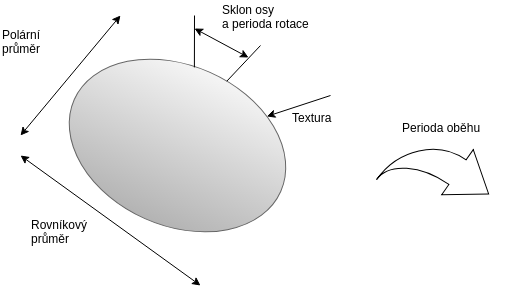
\includegraphics[width=370pt]{Images/BodyData.png}
\caption[Jednoznačná definice tělesa]{Jednoznačná definice tělesa \footnotemark[1]}
\end{center}
\end{figure}

\footnotetext[1]{Vytvořeno v \url{https://www.draw.io}.}

\subsubsection{Orbita}

Orbita je objekt s geometrií \textit{THREE.BufferGeometry}, jejíž tvar je vypočten na základě nejbližší vzdálenosti tělesa od těžiště (pericentrum), nejvzdálenější vzdálenosti tělesa od těžiště (apocentrum) a~výstřednosti dráhy (excentricita). Pro materiál je použit\newline \textit{THREE.LineMaterial} s jedinou barvou namísto textury.

\lstinputlisting[caption={Výpočet geometrie orbity tělesa}, language={JavaScript}]{SourceCodes/Orbit.js}


\begin{figure}[H]
\begin{center}
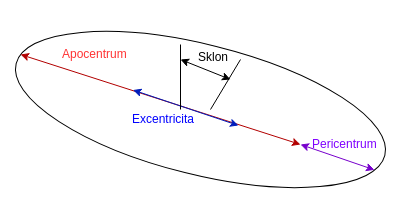
\includegraphics[width=300pt]{Images/OrbitData.png}
\caption[Jednoznačná definice orbity tělesa]{Jednoznačná definice orbity tělesa \footnotemark[1]}
\end{center}
\end{figure}


\subsubsection{Světlo}

Pokud je těleso zdrojem světla, je mezi jeho potomky navíc také bodové světlo\newline \textit{THREE.PointLight}, které emituje světlo o~stejné barvě a~intenzitě, jakou má reálné těleso.

\subsubsection{Prstence}

Prstenec je objekt s~geometrií \textit{THREE.BufferRingGeometry}, materiálem\newline \textit{THREE.MeshLambertMaterial} a~2D~texturou \textit{THREE.Texture} ve formátu \textit{JPG} nebo \textit{PNG}. Těleso může mít libovolný počet prstenců, nebo také žádný.

\begin{figure}[H]
\begin{center}
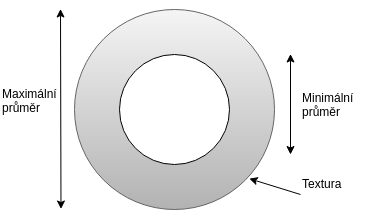
\includegraphics[width=300pt]{Images/RingData.png}
\caption[Jednoznačná definice prstence tělesa]{Jednoznačná definice prstence tělesa \footnotemark[1]}
\end{center}
\end{figure}

\footnotetext[1]{Vytvořeno v \url{https://www.draw.io}.}

\subsubsection{Popisek}

Popisek je reprezentován \textit{HTML} elementem, který je absolutně pozicován na stejné souřadnice, jako je vykreslované těleso. Kromě názvu tělesa obsahuje i~vzdálenost od Země a~vzdálenost od kamery.

\subsection{Serverová část}

\subsubsection{Zachycení HTTP požadavku}

Server vystavuje \textit{REST~API}, ze kterého si mohou klientské aplikace (v~tomto případě pouze webová aplikace) stahovat data. Rozhraní má jasně danou strukturu a~jeho implementace a~dokumentace je provedena pomocí nástroje \textit{Swagger}. Ten umožňuje sestavit rozhraní z~fyzických souborů. Cesta k~souboru značí adresu \textit{URI} a~obsah zas dostupné metody.

\lstinputlisting[caption={Definice cesty v REST~API}, language={JavaScript}]{SourceCodes/Route.js}

Dokumentace je zpřístupněna na lokální adrese \textit{/api-docs}. Je možné se zde informovat o~všech možných \textit{HTTP} požadavcích nebo je s~nastavenými parametry simulovat.

\subsubsection{Zpracování HTTP požadavku}

Jakmile je přijat požadavek od klienta, musí dojít k následujícím krokům:

\begin{itemize}
\item Zjištění identity uživatele z~tokenu v~hlavičce,
\item Zkontrolování vyžadovaných oprávnění,
\item Obsluha požadavku (načtení a zpracování dat z~DB, ...),
\item Nastavení HTTP statusu, popř. chybového kódu,
\item Odeslání odpovědi.
\end{itemize}

V~aplikaci byla vyvinuta vlastní knihovna, která všechny ze zmíněných procesů automatizuje. Pro většinu druhů zdrojů stačí dva druhy přístupových bodů:

\begin{itemize}
\item Pro všechny zdroje,

\begin{itemize}
\item \textbf{GET}: Vrátí pole zdrojů,
\item \textbf{POST}: Vytvoří nový zdroj a~vrátí zprávu o úspěchu nebo chybě,
\item \textbf{DELETE}: Smaže všechny zdroje a~vrátí počet smazaných zdrojů,
\end{itemize}

\item Pro jeden zdroj,

\begin{itemize}
\item \textbf{GET}: Vrátí jeden zdroj podle ID nebo zprávu o~chybě,
\item \textbf{PUT}: Upraví jeden zdroj podle ID a~vrátí zprávu o~úspěchu nebo chybě,
\item \textbf{DELETE}: Smaže jeden zdroj podle ID a vrátí zprávu o úspěchu nebo chybě.
\end{itemize}

\end{itemize}

Samotná definice přístupových bodů pak může vypadat následovně. U každé přístupové metody je možné určit, jaká oprávnění musí mít uživatel, aby tuto metodu nad daným zdrojem mohl vykonat.

\lstinputlisting[caption={Zpracování HTTP požadavku}, language={JavaScript}]{SourceCodes/RouteUtils.js}

Modelové třídy většiny entit není nutné psát individuálně. Všechny mají za úkol poskytnout \textit{CRUD operace} nad danou entitou (např. \textit{BodyModel} nad tělesy). Jediné, co se liší, je název databázové kolekce, vybrané sloupce při výpisu detailu entity a~při výpisu všech entit, popř. další parametry. Veškerá logika komunikace s~databází byla ukryta do třídy \textit{ItemModel}. Většina dalších modelů je pak pouhou instancí této třídy s~konkrétními parametry. \textit{ItemModel} vedle \textit{CRUD} operací automatizuje i vytváření notifikací a~schvalovací proces administrátora.

\lstinputlisting[caption={Automatizovaná tvorba modelových tříd}, language={JavaScript}]{SourceCodes/Model.js}

\subsection{Databáze}

Data v~aplikace se ukládají do databáze \textit{MongoDB} za využití knihovny \textit{Mongoose}. Serverová část se řídí architekturou MVC a~k~databázi mají tedy přístup pouze modelové třídy.

\subsubsection{Připojení do databáze}

Připojení do databáze je jednoznačně inicializováno textovým řetězcem obsahujícím jméno a~heslo uživatele, cluster a~název databáze. Dále je třeba zaregistrovat všechna schémata, která budou v~aplikaci využita. Pokud kolekce s nově zaregistrovaným schématem neexistuje, dojde k jejímu automatickmu vytvoření. Je také možné reagovat na úspěšné připojení nebo na chybu.

Veškerou tuto funkcionalitu obstarává třída \textit{Database}, která byla vytvořena v~rámci projektu. Instance této třídy je staticky (tedy pouze jednou, při spuštění serveru) vytvořena ve třídě \textit{Model}, který je předkem všech ostatních modelových tříd. Třída \textit{Model} pak tuto instanci databáze poskytuje jako instanční proměnnou s~modifikátorem přístupu \code{protected} všem svým potomkům.

\lstinputlisting[caption={Připojení k databázi v~aplikaci}, language={JavaScript}]{SourceCodes/DatabaseConnection.js}

\subsubsection{Mongoose schéma}

Pomocí schématu lze určit strukturu databázové kolekce a nastavit validační pravidla. Veškerá konfigurace je umístěna v~objektu, který se dosadí jako parametr při vytváření nové instance schématu. Je možné také zajistit např. unikátní kombinaci hodnot více polí.

\lstinputlisting[caption={Vytvoření databázového schématu}, language={JavaScript}]{SourceCodes/Schema.js}

\subsubsection{Mongoose plugin}

Pokud je třeba reagovat na jednotlivé události v kolekci (smazání, vložení, ...), lze toho docílit pomocí pluginů. To jsou obdoby spouští z relačních databází. Jedná se o~uživatelem definované funkce, které dostanou v~parametru schéma, na kterém jsou zaregistrovány. Na tomto schématu pak mohou definovat operace \code{pre} nebo \code{post} s~jednotlivými událostmi a~jejich obsloužení.

\lstinputlisting[caption={Vytvoření a~použití databázového pluginu}, language={JavaScript}]{SourceCodes/Hash.js}

Ve zdrojovém kódu~12 je zobrazena část pluginu pro automatické hashování hesla. Ten při každé změně daného pole nový obsah zahashuje a~teprve onen hash uloží do databáze namísto původní hodnoty. Protože ale není vyloučené, že bude někdy třeba tento plugin použít také v~jiném schématu a~na jiném poli, plugin byl vytvořen univerzálně. Jméno pole je proto určeno parametrem v~pluginu.

\subsubsection{Základní práce s databází}

Databáze umožňuje provádět velké množství operací nad daty v~ní uloženými. Je možné vyhledávat podle konkrétní hodnoty, pole hodnot, regulárních výrazů nebo číselného rozsahu. Takto vyfiltrovaná data lze číst, smazat či editovat. Je také možné nastavit spoustu parametrů, např. maximální počet dokumentů (\textit{limit}), které vyhovují filtru. Mimo jiné je možné také provádět více dotazů do databáze jako atomické operace pomocí transakcí.

\lstinputlisting[caption={CRUD operace nad kolekcí uživatelů}, language={JavaScript}]{SourceCodes/Database.js}

\subsubsection{Aggregation Framework}

V případě složitějších databázových dotazů, na které nestačí předpřipravené metody knihovny \textit{Mongoose}, je možno využít metodu \code{aggregate}, jež umožňuje pracovat s~\textit{Aggregation Frameworkem} databáze \textit{mongoDB}. Ten mimo jiné umožňuje v tzv. \textit{pipeline} dosadit sekvenci dotazů, které se nad daty postupně provedou. Je tak možné používat např. \code{\$match} (vyhledávání), \code {\$group} (seskupování) nebo \code{\$lookup} (spojování více kolekcí).

V~aplikaci je tento způsob dotazování použit např. při požadavku \code{[GET] /bodies/{bodyId}}, kdy je třeba z~databáze kromě tělesa na základě jeho ID vybrat z jiných kolekcí i typ tělesa, události v~historii tělesa, diskuse o~tělese, komentáře k~diskusím a~nakonec i~uživatele a~hlasy patřící k~jednotlivým diskusím a~komentářům. Konkrétní podoba dotazu použitého v~aplikaci je zobrazena v~příloze~B~na konci tohoto dokumentu.

\section{Rozvržení aplikace}

\subsection{Hlavní stránka}

Hlavní stránka aplikace obsahuje pouze nezbytné odkazy do dalších částí aplikace. Nepřihlášený vidí odkazy do simulátoru a~přihlašovací stránku. Přihlášený uživatel vidí taktéž odkaz do simulátoru, ale druhé tlačítko slouží pro odhlášení.

\begin{figure}[H]
\begin{center}

\includegraphics[width=450pt]{Images/MainPage.png}
\caption{Hlavní stránka}
\label{BodiesList}
\end{center}
\end{figure}

\subsection{Nápověda}

V~nápovědě je shromážděno několik článků, které mohou pomoci novým uživatelům lépe se orientovat v~aplikaci. Mezi jednotlivými sekcemi nápovědy lze přepínat pomocí menu v~levé části obrazovky.

\subsection{Autentifikace uživatele}

\subsubsection{Identita}

Každý uživatel, jenž se chce přihlásit nebo se zaregistrovat, se dostane na stránku, kde musí prokázat svou identitu zadáním emailu. V~závislosti na tom, zda zadaný email již v~databázi existuje bude odkázán na stránku pro přihlášení nebo pro registraci.

\begin{figure}[H]
\begin{center}

\includegraphics[width=250pt]{Images/Identity.png}
\caption{Formulář pro zjištění identity uživatele}
\label{Identity}
\end{center}
\end{figure}

\subsubsection{Přihlášení}

Stránka obsahuje formulář pro zadání hesla. Nachází se zde odkaz zpět a~odkaz pro obnovení hesla.

\begin{figure}[H]
\begin{center}
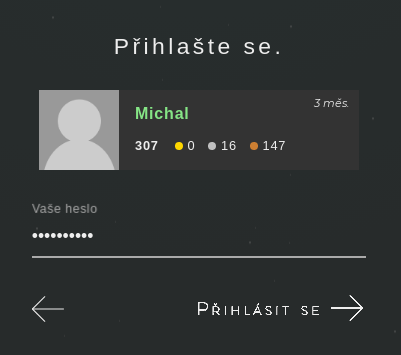
\includegraphics[width=250pt]{Images/SignIn.png}
\caption{Formulář pro přihlášení uživatele}
\label{SignIn}
\end{center}
\end{figure}

\subsubsection{Registrace}

Stránka pro zadání a potvrzení hesla k nově vytvářenému účtu. V~případě, že uživatel chce změnit registrační email, je možné se vrátit na stránku se zadáváním identity.

\begin{figure}[H]
\begin{center}

\includegraphics[width=250pt]{Images/SignUp.png}
\caption{Formulář pro registraci uživatele}
\label{SignUp}
\end{center}
\end{figure}

\subsubsection{Zapomenuté heslo}

Na této stránce se nachází formulář s~polem pro email. Po úspěšném vyplnění se odešle na zadaný email zpráva s~odkazem pro obnovení hesla.

\subsubsection{Reset hesla}

Stránka obsahuje formulář pro nastavení a~potvrzení nového hesla. Pro úspěch je nutné, aby se v~URL adrese nacházel platný token. Ten se vytvoří v okamžiku vytvoření požadavku na obnovu hesla a~má platnost 30 minut.

\subsection{Uživatel}

\subsubsection{Detail uživatele}

\subsubsection{Editace uživatele}
	
\subsection{Simulátor}

Hlavní náplní aplikace je právě tato stránka. Na 3D scéně zobrazuje tělesa ve vesmíru v~reálném čase s realistickými poměry velikostí i~vzdáleností. Uživatel může myší nebo touchpadem libovolně otáčet kamerou kolem vycentrovaného tělesa.

V~pravém dolním rohu se nachází ovládací panel, jenž umožňuje měnit některá nastavení simulátoru. Všechna z~nich jsou dostupná i~pod klávesovými zkratkami.

\begin{itemize}
\item \textbf{Jména} (N): Zobrazí nebo skryje názvy těles.
\item \textbf{Vzdálenosti od kamery} (C): Zobrazí nebo skryje vzdálenosti těles od kamery.
\item \textbf{Vzdálenosti od Země} (E): Zobrazí nebo skryje vzdálenosti těles od Země.
\item \textbf{Zrychlit} (W): Pokud je čas kladný, zrychlí ho 10krát. Jinak ho 10krát zpomalí.
\item \textbf{Zpomalit} (S): Pokud je čas kladný, zpomalí ho 10krát. Jinak ho 10krát zrychlí.
\item \textbf{Vrátit čas} (T): Nastaví čas simulátoru na aktuální čas.
\item \textbf{Vrátit rychlost} (V): Nastaví čas simulátoru na 1.
\item \textbf{Panel} (P): Zobrazí nebo skryje detail právě vycentrovaného tělesa.
\item \textbf{Pohyb} (M): Spustí nebo ukončí rotaci kamery kolem vycentrovaného tělesa.
\item \textbf{Světlo} (L): Zapne nebo vypne světlo.
\item \textbf{Orbity} (O): Zobrazí nebo skryje orbity těles.
\end{itemize}

Na dolním okraji obrazovky je lišta zobrazující aktuální nastavení a~čas simulátoru. Napravo je možné vidět posuvník s aktuální velikostí pohledu.

\begin{figure}[H]
\begin{center}
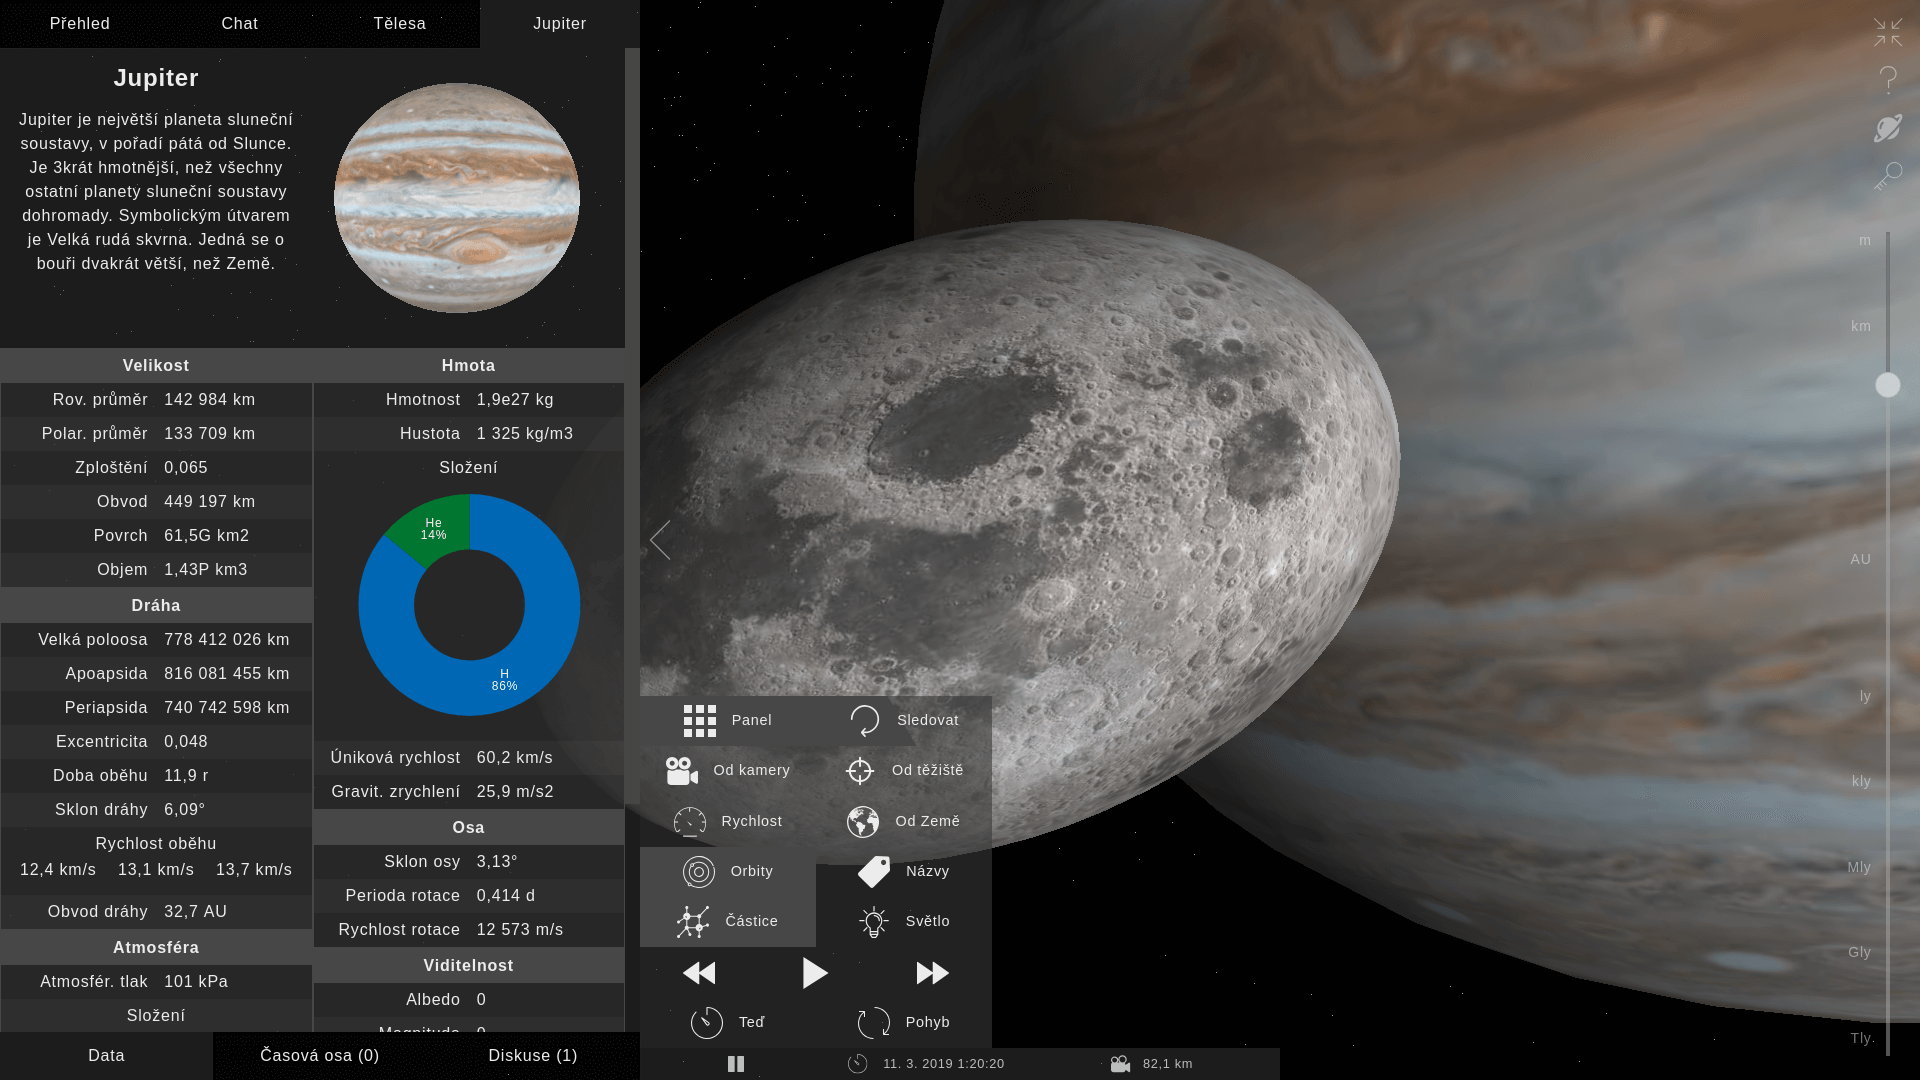
\includegraphics[width=450pt]{Images/Simulator.png}
\caption{Simulátor}
\label{BodiesList}
\end{center}
\end{figure}

\subsection{Uživatelský panel}

Uživatelský panel je sekundární okno, ve kterém si uživatel může zobrazovat části aplikace bez nutnosti opouštět aktuální stránku. Zobrazuje se jako poloprůhledný obdélník v levé části obrazovky a obsahuje 4~nezávislé záložky.

\subsubsection{Přehled}

Výchozí položka v~uživatelském panelu zobrazuje poslední události na webu a~uživatele. Uživatele lze řadit podle času poslední aktivity nebo reputace. Přihlášený uživatel zde také vidí stručné informace o~svém účtu.

\begin{figure}[H]
\begin{center}
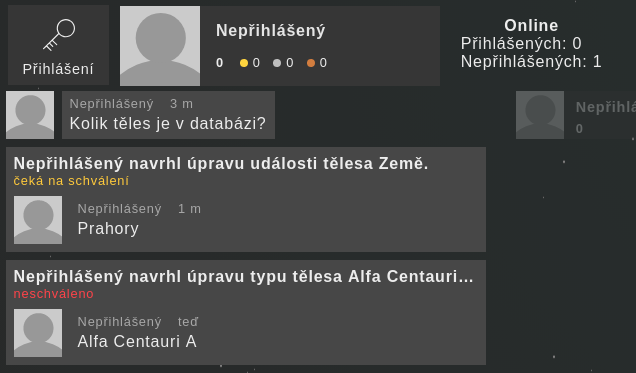
\includegraphics[width=350pt]{Images/Overview.png}
\caption{Přehled}
\label{BodiesList}
\end{center}
\end{figure}

\subsubsection{Chat}

Chat slouží pro vzájemnou komunikaci uživatelů. Zprávy jsou zobrazovány okamžitě všem aktivním uživatelům díky technologii \textit{socket.io}.

\begin{figure}[H]
\begin{center}
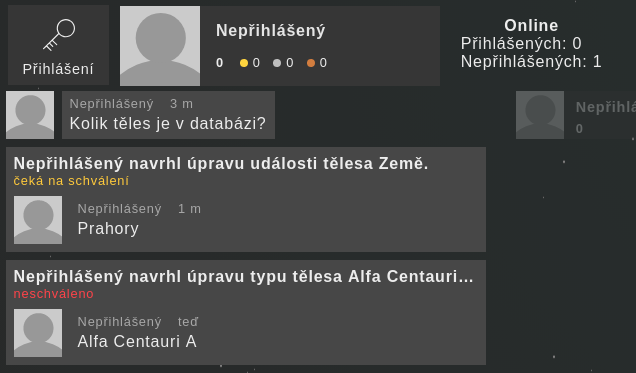
\includegraphics[width=350pt]{Images/Overview.png}
\caption{Uživatelský chat}
\label{BodiesList}
\end{center}
\end{figure}


\subsubsection{Seznam těles}

Seznam těles umožňuje zobrazit tělesa v~databázi i~s~jejich údaji. Údaje mohou být:

\begin{itemize}
\item \textbf{Absolutní}: Zobrazí absolutní hodnotu (např. průměr Slunce je 1~392~684~km).
\item \textbf{Relativní k libovolnému tělesu}: Zobrazí poměr aktuální hodnoty ku hodnotě u~porovnávaního tělesa (např. průměr Slunce je roven 109~průměrům Země).
\end{itemize}

Tělesa lze řadit vzestupně i~sestupně podle libovolného kritéria a~taktéž je lze podle libovolných kritérií filtrovat za použití následujících vztahů:

\begin{itemize}
\item \textbf{Obsahuje}: Vyhoví, pokud hodnota obsahuje hledaný text.
\item \textbf{Je roven}: Vyhoví, pokud je hodnota rovna hledanému textu.
\item \textbf{Začíná na}: Vyhoví, pokud hodnota začíná hledaným textem.
\item \textbf{Končí na}: Vyhoví, pokud hodnota končí hledaným textem.
\item \textbf{Je větší než}: Vyhoví, pokud je hodnota větší, než hledaný text. V~případě nečíselné hodnoty vyhoví ty, které se v~abecedě nachází později.
\item \textbf{Je menší než}: Vyhoví, pokud je hodnota menší, než hledaný text. V~případě nečíselné hodnoty vyhoví ty, které se v~abecedě nachází dříve.
\end{itemize} 

\begin{figure}[H]
\begin{center}
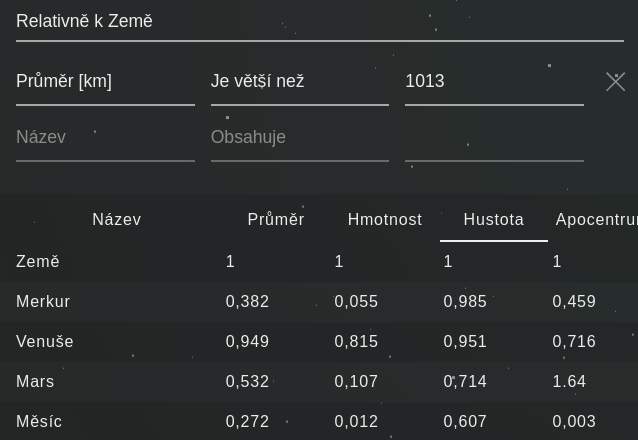
\includegraphics[width=350pt]{Images/Bodies.png}
\caption{Seznam těles}
\label{BodiesList}
\end{center}
\end{figure}

\subsubsection{Detail tělesa}

Detail tělesa se skládá ze čtyř záložek. Výchozí z nich zobrazuje výčet všech známých údajů v~tabulce o~daném tělese. Součástí je i~krátká charakteristika tělesa a~jeho 3D vizualizace.

Na druhé záložce se nachází časová osa, na které jsou vyneseny historické události spojené s~tělesem. Každá událost obsahuje rok, ve kterém nastala, název a~po najetí kurzorem  i~krátký popis. Je zde i stručný graf zobrazující počet výskytů události v~jednotlivých časových obdobích.

Třetí záložka je určena pro diskuse. Každý zde může reagovat na již existující diskuse, nebo může založit vlastní vlákno. Všechny příspěvky uživatelů lze kladně nebo záporně hodnotit, v důsledku čehož se bude přičítat nebo odečítat reputace autora.

\begin{figure}[H]
\begin{center}
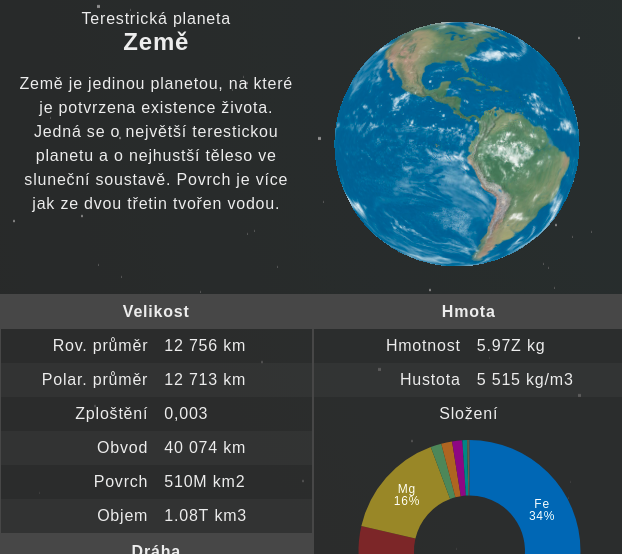
\includegraphics[width=350pt]{Images/Body.png}
\caption{Detail tělesa}
\label{BodiesList}
\end{center}
\end{figure}

\begin{figure}[H]
\begin{center}
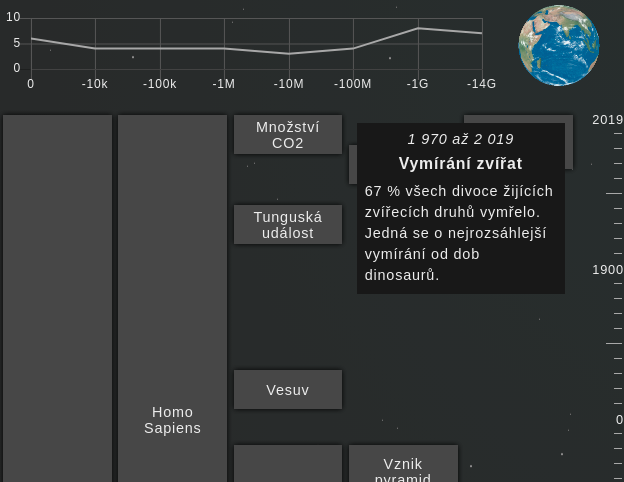
\includegraphics[width=350pt]{Images/Timeline.png}
\caption{Časová osa tělesa}
\label{BodiesList}
\end{center}
\end{figure}

\begin{figure}[H]
\begin{center}
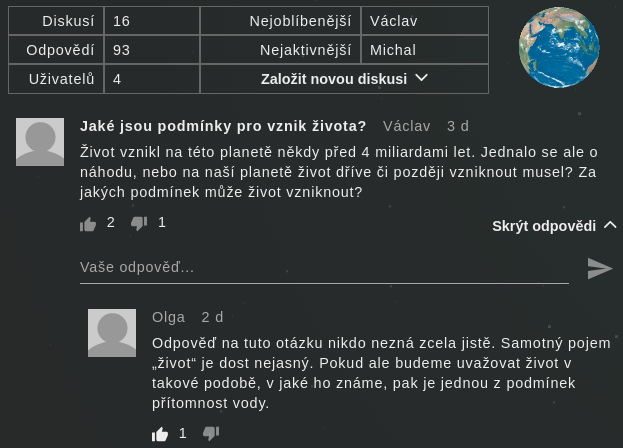
\includegraphics[width=350pt]{Images/Discussion.png}
\caption{Diskuse o tělese}
\label{BodiesList}
\end{center}
\end{figure}

\section{Problémy řešené při implementaci}

\subsection{Omezení viditelnosti těles}

V~databázi je uloženo velké množství těles. Pokud by se popisky a~dráhy všech těles zobrazovaly najednou, bylo by těžké se v simulátoru orientovat. Navíc by tento stav měl negativní důsledky na výkon aplikace. Proto se ve vykreslovací smyčce počítá relativní poloha všech těles vzhledem ke kameře. V~závislosti na této poloze se určí, jak se bude dané těleso zobrazovat. Může nastat několik případů, které je nutno ošetřit:

\begin{itemize}
\item \textbf{Dráha je 40krát větší/menší než obrazovka}: Dráha tělesa bude poloprůhledná, popisky se nebudou zobrazovat.
\item \textbf{Dráha je 1000krát větší/menší než obrazovka}: Dráha ani popisky se nebudou zobrazovat.
\item \textbf{Vzdálenost od tělesa je 40krát větší než vzdálenost od centrálního tělesa}: Dráha tělesa bude poloprůhledná, popisky se nebudou zobrazovat.
\item \textbf{Vzdálenost od tělesa je 1000krát větší než vzdálenost od centrálního tělesa}: Dráha ani popisky se nebudou zobrazovat.
\end{itemize} 

První dva body řeší případy, kdy je těleso příliš oddálené nebo příliš přiblížené. Poslední dva body řeší situaci, ve které má uživatel sice přiměřené přiblížení kamery, nicméně se od tělesa nachází příliš daleko. Příkladem může být situace, kdy si uživatel prohlíží ze vzdálenosti 400~tisíc km prstence planety Saturn. Dráha zemského Měsíce je přiměřeně velká (406~tisíc km), ale přesto by se neměla vykreslovat. Od Saturnu je totiž vzdálena 1,2~miliardy km.

\subsection{Sestavení aplikace a~optimalizace}

\begin{figure}[H]
  \centering
  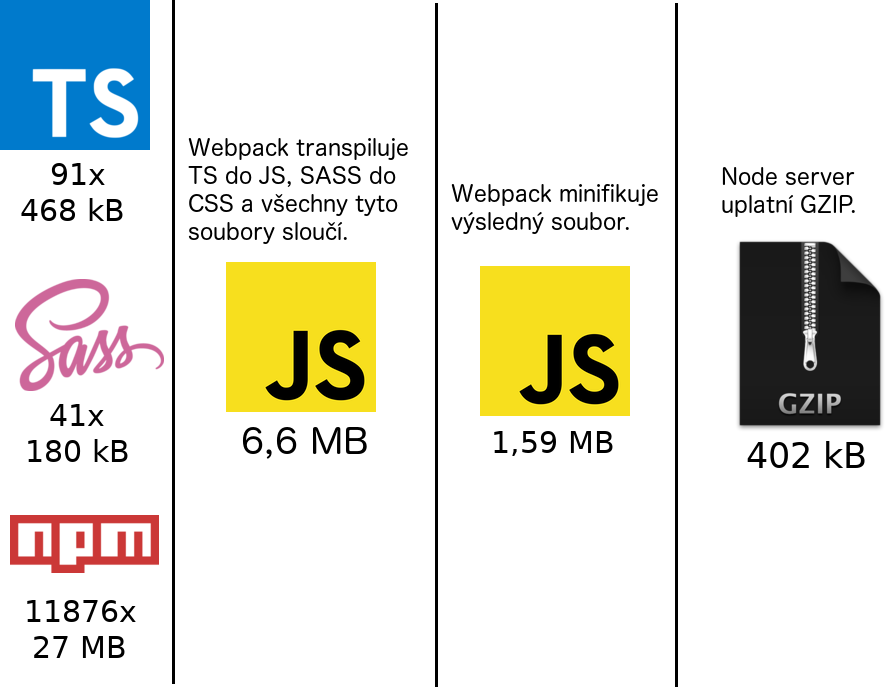
\includegraphics[width=280pt]{Images/Webpack.png}
  \caption[Sestavení aplikace a~optimalizace]{Sestavení aplikace a~optimalizace   \footnotemark[1]\textsuperscript{, }\footnotemark\textsuperscript{, }\footnotemark}
\end{figure}

\footnotetext[1]{Ikona SASS převzata z \url{https://sass-lang.com/assets/img/logos/logo-b6e1ef6e.svg}}
\footnotetext[2]{Ikona NPM převzata z \url{https://pepa.holla.cz/wp-content/uploads/2016/06/npm.png}}
\footnotetext[3]{Ikona GZIP převzata z \url{https://codeopinion.com/wp-content/uploads/2016/02/gzip.png}}

\subsubsection{Transpilace a~sloučení JS a~CSS souborů}

V~projektu se nachází velké množství souborů s~typescriptovým kódem a~souborů se styly. Zahajovat HTTP požadavek pokaždé, kdy si uživatel chce stáhnout jakýkoliv z~těchto souborů vyžaduje hodně režije a je to z~hlediska času i~přenesených dat náročné. Je proto výhodnější všechny tyto soubory sloučit do jediného a~ten stáhnout jako jeden celek.

Ze všeho nejdříve je ale nutné transpilovat zdrojové kódy do nativních jazyků. Prohlížeče totiž TypeScriptu ani SASSu nerozumí. TypeScript se transpiluje do JavaScriptu za využití transpilátoru, jenž je dodáván společně s~TypeScriptem. Pro převod SASS na CSS slouží Webpack. Ten následně také všechny takto transpilovaného soubory slouží do jediného javascriptového souboru.

\subsubsection{Minifikace a~GZIP komprese}

I přesto, že jsou všechny zdrojové soubory sloučené do jednoho, stále se jedná o~velký objem dat. Je proto vhodné celý soubor pomocí nástroje Webpack minifikovat~–~odebrat z~něj přebytečné mezery, komentáře a~zkrátit názvy lokálních proměnných.

Pro ještě větší redukci přenesených dat je dobré nastavit Node.js server tak, aby na všechny odeslané soubory uplatnil GZIP kompresi.

\subsection{Bezpečnost a~ochrana dat}

\subsubsection{Autentizace pomocí tokenu}

Uživatel se autentizuje při přihlášení svým emailem a heslem, čímž mu je umožněn přístup na jeho účet. Nicméně uživatele je třeba znovu autentizovat i~během jeho relace po přihlášení, kdykoliv komunikuje se serverem. Tím lze omezit provádění určitých operací (např. editování tělesa, schvalování úprav, ...) pouze na konkrétní uživatele nebo skupiny uživatelů (např. pouze přihlášení, administrátoři, ...). Nabízí se několik možností v tom, co na server posílat vždy, když je třeba autentifikace:

\begin{itemize}
\item \textbf{Email a heslo}: Nechat uživatele zadávat přihlašovací údaje pokaždé, když je třeba komunikovat se serverem, by bylo obtěžující. A~ukládat heslo na straně klienta není zas bezpečné, protože by zde muselo být v~čitelné podobě.

\item \textbf{ID uživatele}: Jedná se o~nebezpečný postup. ID uživatele je veřejný údaj, ke kterému mají přístup i~všichni ostatní. Nic by tedy nebránilo útočníkovi poslat \textit{HTTP} požadavek s~ID libovolného uživatele.

\item \textbf{Token}: Ideálním způsobem se zdá být vygenerování pseudonáhodného textového řetězce při přihlášení. Tímto řetězcem se po dobu přihlášení bude uživatel prokazovat. Protože tento řetězec nezná nikdo jiný, než uživatel sám, nikdo jiný se s~ním tedy nemůže autentizovat. Navíc proti zneužití má omezenou platnost, po jejímž vypršení je třeba požádat o~nový token.
\end{itemize}

V~aplikaci je využit poslední ze zmíněných způsobů. Token má platnost 30 minut. Je tedy zajištěna bezpečná autoritace. Každý může provádět pouze ty operace, na které má~skutečně právo.

\subsubsection{Hashování hesel}

Ukládat hesla v čitelné podobě do databáze není bezpečné. Potenciální útočník, který by prolomil zabezpečení serveru a~dostal se k~databázi by viděl hesla všech uživatelů. Tento problém řeší \textit{hashování hesel}.

Do databáze se neuloží heslo samotné, ale pouze jeho otisk (\textit{hash}). Když je potřeba porovnat zadané heslo (např. při přihlášování) s heslem, porovnají se jejich otisky. Tím je umožněna autentifikace a~zároveň je znemožněno útočníkovi přečíst hesla z~databáze.

Pro vyšší bezpečnost se otisk nevypočítává z pouhého hesla, ale hesla spojeného s~dalším nijak nesouvisejícícm řetězcem. Tím se zabrání možnosti, aby více uživatelů mělo stejné heshe, pokud mají stejná hesla. Tomuto dodatečnému řetězci se říká sůl (\textit{salt}). Často se také otisk vypočítává několikrát za sebou, takže v databázi není uložen otisk hesla, ale otisk, který vznikl na základě jiného otisku.

\textit{Hash} je výsledkem jednosměrné funkce. To znamená, že z již vypočteného hashe nelze získat původní text. Výjimku tvoří zastaralé \textit{hashovací} funkce, které již byly prolomeny. Je vytvořena databáze pro všechny možné otisky a~texty, ze kterých byly vypočítány.

V~aplikaci je použita \textit{hashovací funkce bcrypt} s~10 iteracemi a~to přímo na úrovni databáze. Celá logika je skryta do tzv. \textit{Mongoose pluginu}. Ten může reagovat na různé události a~modifikovat dokument.

\lstinputlisting[caption={Hashování hesel v Mongoose schématu}, language={JavaScript}]{SourceCodes/Hash.js}

\subsection{Zobrazování hodnot fyzikálních veličin}

Aplikace zobrazuje různě velké hodnoty různých fyzikálních veličin. Z~důvodu přehlednosti a~omezeného množství prostoru, ve kterém se tyto hodnoty zobrazují, byla vytvořena pomocná třída \code{Units} umístěná do modulu \code{Utils}. Ta umožňuje převádět a~formátovat jednotky do několika podob.

\lstinputlisting[caption={Ukázka formátování jednotek}, language={JavaScript}]{SourceCodes/Units.js}

Všechny číselné hodnoty se automaticky zaokrouhlují s~rozumnou přesností:

\lstinputlisting[caption={Ukázka zaokrouhlování hodnot}, language={JavaScript}]{SourceCodes/Round.js}

Není nutné používat předdefinované jednotky v~této třídě a~lze si vytvořit vlastní. Vytvoření jednotek pro velikost vypadá takto:

\lstinputlisting[caption={Tvorba vlastních jednotek}, language={JavaScript}]{SourceCodes/CreateUnits.js}

\subsection{Vykreslování časové osy}

Pro vykreslení časové osy představené v~bodě \textit{4.5.4~Detail tělesa} byla v~rámci projektu vytvořena komponenta \textit{EventsArea}. Ta umožňuje vykreslit pole událostí na \textit{2D} ploše v~podobě čtyřúhelníků tak, aby si souřadnice jednotlivých událostí odpovídaly. V~případě časové osy jsou těmito souřadnicemi počáteční a~koncový rok události.

Situace je o~to komplikovanější, že časová osa nemusí být lineární a~dokonce ani logaritmická. Komponenta proto na vstupu vedle pole událostí přijme i~pole hraničních souřadnic. Díky tomu je možné zobrazit roky 2019 až 0 jako jeden díl na časové ose a~o~něco níže naprosto stejný díl pro roky -1 až -10~000, stejně jako např. -5~mld. až -10~mld.

Překrývání jednotlivých události je ošetřeno tak, že se vykreslí do různých sloupců. Je také možno nastavit počet mezistupňů mezi hraničními souřadnicemi. Ty lze nastylovat např. jako čáry na pravítku pro zlepšení přehlednosti. Při pohybu s kurzorem myši nad oblastí se zobrazuje horizontální čára s aktuální souřadnicí (rokem), nad kterou se kurzor nachází. Pro implementaci komponenty byla použita \textit{CSS} vlastnost \textit{grid}.

\lstinputlisting[caption={Příklad použití komponenty EventsArea}, language={JavaScript}]{SourceCodes/EventsArea.js}


%%%%%%%%%%%%%%%%%%%%%%%%%%%%%%%%%%%%%%%%%%%%%%%%%%%%%%%%%%%%
% ZÁVĚR
%%%%%%%%%%%%%%%%%%%%%%%%%%%%%%%%%%%%%%%%%%%%%%%%%%%%%%%%%%%%

\clearpage \phantomsection \addcontentsline{toc}{section}{Závěr}
\section*{Závěr}


%%%%%%%%%%%%%%%%%%%%%%%%%%%%%%%%%%%%%%%%%%%%%%%%%%%%%%%%%%%%
% POUŽITÁ LITERATURA
%%%%%%%%%%%%%%%%%%%%%%%%%%%%%%%%%%%%%%%%%%%%%%%%%%%%%%%%%%%%

\clearpage \phantomsection \addcontentsline{toc}{section}{\refname}

\begin{thebibliography}{99}	% parametr určuje nejširší položku

% nezlomitelné spojovníky lze zapisovat zkratkou "- nebo příkazem \babelhyphen{nobreak}

\bibitem{kleczek}
KLECZEK, Josip. Velká encyklopedie vesmíru. Praha: Academia, 2002s [cit. 25. 10. 2018]. ISBN 80-200-0906-x.

\bibitem{rees}
REES, Martin, Vesmír. Přeložil Pavel PŘÍHODA. Praha: Knižní klub, 2006 [cit. 25. 10. 2018]. ISBN 80-242-1668-x.

\bibitem{jpl}
JPL Solar System Dynamics. \textit{JPL Solar System Dynamics} [online]. [cit. 25. 10. 2018] Dostupné z: \url{https://ssd.jpl.nasa.gov}.

\bibitem{mardan}
MARDAN, Azat. Practical Node.js: building real-world scalable web apps. Berkeley, California: Apress, [2014]. Expert‘s voice in Web development. ISBN 978-1-4302- 6595-5.

\bibitem{banks}
BANKS, Alex and PORCELLO, Eve. Learning React: functional web development with React and Redux. Sebastopol, CA: O'Reilly Media, 2017 [cit. 25. 10. 2018]. ISBN: 978-1-4919-542-1.

\bibitem{typescript}
TypeScript. 
\textit{TypeScript.} [online]. [cit.\,22.~2~2019]. 
Dostupné\newline z:~{\ttfamily \url{https://www.typescriptlang.org}}.

\bibitem{react}
React. 
\textit{React.} [online]. [cit.\,22.~2.~2019]. 
Dostupné\newline z:~{\ttfamily \url{https://reactjs.org}}.

\bibitem{virtualdom}
React: The Virtual DOM.
\textit{codeacademy.} [online]. [cit.\,22.~2.~2019]. 
Dostupné\newline z:~{\ttfamily \url{https://www.codecademy.com/articles/react-virtual-dom}}.

\bibitem{onewaydatabinding}
Thinking in React.
\textit{React.} [online]. [cit.\,22.~2.~2019]. 
Dostupné\newline z:~{\ttfamily \url{https://reactjs.org/docs/thinking-in-react.html}}.

\bibitem{jsxsyntax}
Introducing JSX. 
\textit{React.} [online]. [cit.\,22.~2.~2019]. 
Dostupné\newline z:~{\ttfamily \url{https://reactjs.org/docs/introducing-jsx.html}}.

\bibitem{node}
MROZEK, Jakub. JavaScript na serveru: Architektura a první Hello World.
\textit{Zdroják.} [online]. 5.~10.~2012. [cit.\,22.~2.~2019].  ISSN 1803-5620.
Dostupné\newline z:~{\ttfamily \url{https://www.zdrojak.cz/clanky/javascript-na-serveru-architektura-a-prvni-hello-world/}}.

\bibitem{three}
BOTMAN, Chris. An introduction to Three.js.
\textit{Humaan.} [online]. 5.~02.~2016. [cit.\,22.~2.~2019].  ISSN 1803-5620.
Dostupné\newline z:~{\ttfamily \url{https://humaan.com/blog/web-3d-graphics-using-three-js/}}.

\bibitem{mongomongoose}
MROZEK, Jakub. JavaScript na serveru: MongoDB, Mongoose a AngularJS.
\textit{Zdroják.} [online]. 26.~10.~2012. [cit.\,22.~2.~2019].  ISSN 1803-5620.
Dostupné\newline z:~{\ttfamily \url{https://www.zdrojak.cz/clanky/javascript-na-serveru-mongodb-mongoose-angularjs/}}.

\bibitem{git}
Úvod - Základy systému Git.
\textit{git.} [online]. [cit.\,22.~2.~2019]. 
Dostupné z: {\ttfamily \url{https://git-scm.com/book/cs/v1/%C3%9Avod-Z%C3%A1klady-syst%C3%A9mu-Git}}.

\bibitem{webpack}
Concepts.
\textit{webpack.} [online]. [cit.\,22.~2.~2019].
Dostupné z: {\ttfamily \url{https://webpack.js.org/concepts}}.

\bibitem{jsconcat}
Fantastic front-end performance.
\textit{HACKS.} [online]. 20~2~2019. [cit.\,22.~2.~2019].
Dostupné z: {\ttfamily \url{https://hacks.mozilla.org/2012/12/fantastic-front-end-performance-part-1-concatenate-compress-cache-a-node-js-holiday-season-part-4/}}.

\bibitem{npm}
MICHÁLEK, Martin. NPM: Průvodce začátky a základními příkazy.
\textit{Vzhůru dolů.} [online]. 19.~11.~2019. [cit.\,22.~2.~2019].
Dostupné z: {\ttfamily \url{https://www.vzhurudolu.cz/prirucka/npm}}.

\end{thebibliography}


%%%%%%%%%%%%%%%%%%%%%%%%%%%%%%%%%%%%%%%%%%%%%%%%%%%%%%%%%%%%
% PŘÍLOHY
%%%%%%%%%%%%%%%%%%%%%%%%%%%%%%%%%%%%%%%%%%%%%%%%%%%%%%%%%%%%


\clearpage \phantomsection \addcontentsline{toc}{section}{Seznam příloh}
\section*{Seznam příloh}

\noindent Příloha~A -- Struktura databáze \dotfill \pageref{prilohaA}

\noindent Příloha~B -- Využití aggregation frameworku \dotfill \pageref{prilohaB}

% PŘÍLOHA A

\clearpage \phantomsection\label{prilohaA} 
% do obsahu i do záložek PDF:
%\addcontentsline{toc}{section}{Příloha~A -- Uvozovky}
% pouze do záložek PDF:
%\pdfbookmark[1]{Příloha~A -- Struktura databáze}{prilohaA}	% záložka do PDF
\section*{Příloha~A --  Struktura databáze}
%\pdfbookmark[1]{Příloha~B -- Využití aggregation frameworku}{prilohaB}	% záložka do PDF
\section*{Příloha~B --  Využití aggregation\newline frameworku}

\lstinputlisting[nolol,language={JavaScript}]{SourceCodes/Aggregation.js}

\clearpage \phantomsection \addcontentsline{toc}{section}{Seznam souborů zdrojových kódů na přiloženém nosiči}
\section*{Seznam souborů zdrojových kódů na přiloženém nosiči}

\noindent Příloha~A \dotfill \pageref{prilohaA}

%%%%%%%%%%%%%%%%%%%%%%%%%%%%%%%%%%%%%%%%%%%%%%%%%%%%%%%%%%%%
% KONEC DOKUMENTU
%%%%%%%%%%%%%%%%%%%%%%%%%%%%%%%%%%%%%%%%%%%%%%%%%%%%%%%%%%%%

\end{document}

% vim:sw=8:ts=8
% EOF
